

\documentclass[paper=b4j,landscape,fontsize=9pt]{jlreq}
\usepackage[divide=3,answer]{itohasheet}
\タイトル{【中間考査　対策プリント】vol.1}



\begin{document}
\setlength{\abovedisplayskip}{2pt} % 数式環境の上の余白
\setlength{\belowdisplayskip}{2pt} % 数式環境の下の余白
\begin{分割}

\begin{問題挿入}[-1]{\themondai}<基本>
  $0^{\circ}\leq \theta\leq 180^{\circ}$のとき，次の方程式を解け。
  \begin{enumerate}[itemsep=0.25\zw]
    \item $\sin{\theta}=\frac{1}{2}$
    \item $\cos{\theta}=-\frac{\sqrt{3}}{2}$
    \item $\tan{\theta}=1$
  \end{enumerate}
\end{問題挿入}
\begin{解答挿入}
  \begin{enumerate}
    \item 下の図から$\theta=30^{\circ},\; 150^{\circ}$.
    \begin{center}
      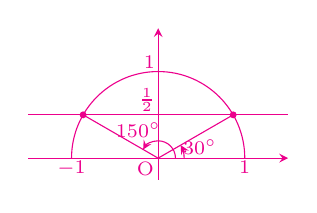
\begin{tikzpicture}[scale=1.1,color=magenta,>=stealth,]
        \node[below left=-2pt,font=\scriptsize] at (0,0){O}; 
        \node[above left,inner sep=1pt,font=\scriptsize] at (0,1){$1$}; 
        \node[below,inner sep=1pt,font=\scriptsize] at (1,0){$1$}; 
        \node[below,inner sep=1pt,font=\scriptsize] at (-1,0){$-1$}; 

        \draw[->] (-1.5,0) -- (1.5,0);
        \draw[->] (0,-0.25) -- (0,1.5);

        \draw (1,0) arc (0:180:1);

        \draw (-1.5,0.5) -- (1.5,0.5) ;
        \node[above left,font=\scriptsize,inner sep=1pt] at (0,0.5){$\frac{1}{2}$};

        \coordinate (P1) at (30:1);
        \coordinate (P2) at (150:1);
        \fill (P1) circle[radius=0.4mm];
        \fill (P2) circle[radius=0.4mm];

        \draw (P1) -- (0,0);
        \draw (P2) -- (0,0);

        \draw[->] (0.3,0) arc (0:30:0.3);
        \draw[->] (0.2,0) arc (0:150:0.2);

        \node[font=\scriptsize]at (15:0.5) {$30^{\circ}$};
        \node[font=\scriptsize]at (125:0.4) {$150^{\circ}$};

      \end{tikzpicture}
    \end{center}
    \item 下の図から$\theta=150^{\circ}$.
    \begin{center}
      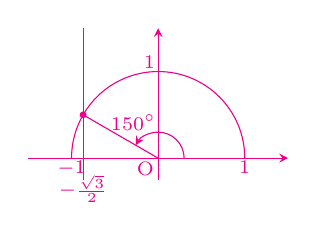
\begin{tikzpicture}[scale=1.1,color=magenta,>=stealth,]
        \node[below left=-2pt,font=\scriptsize] at (0,0){O}; 
        \node[above left,inner sep=1pt,font=\scriptsize] at (0,1){$1$}; 
        \node[below,inner sep=1pt,font=\scriptsize] at (1,0){$1$}; 
        \node[below,inner sep=1pt,font=\scriptsize] at (-1,0){$-1$}; 

        \draw[->] (-1.5,0) -- (1.5,0);
        \draw[->] (0,-0.25) -- (0,1.5);

        \draw (1,0) arc (0:180:1);

        \draw ({-0.5*sqrt(3)},1.5) -- ({-0.5*sqrt(3)},-0.25) node[below,inner sep=-2pt,font=\scriptsize]{$-\frac{\sqrt{3}}{2}$};

                
        \coordinate (P1) at (150:1);
        \fill (P1) circle[radius=0.4mm];

        \draw (P1) -- (0,0);

        \draw[->] (0.3,0) arc (0:150:0.3);

        \node[font=\scriptsize]at (125:0.5) {$150^{\circ}$};

      \end{tikzpicture}
    \end{center}
    \item 下の図から$\theta=45^{\circ}$.
    \begin{center}
      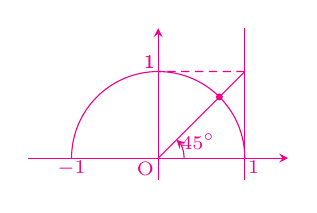
\begin{tikzpicture}[scale=1.1,color=magenta,>=stealth,]
        \node[below left=-2pt,font=\scriptsize] at (0,0){O}; 
        \node[above left,inner sep=1pt,font=\scriptsize] at (0,1){$1$}; 
        \node[below right,inner sep=1pt,font=\scriptsize] at (1,0){$1$}; 
        \node[below,inner sep=1pt,font=\scriptsize] at (-1,0){$-1$}; 

        \draw[->] (-1.5,0) -- (1.5,0);
        \draw[->] (0,-0.25) -- (0,1.5);

        \draw (1,0) arc (0:180:1);

        \draw (1,1.5) -- (1,-0.25);

        \coordinate (P1) at (1,1);
        \draw[densely dashed] (P1) -- (0,1) node[above left,inner sep=1pt,font=\scriptsize]{$1$};

        
        \fill (45:1) circle[radius=0.4mm];

        \draw (P1) -- (0,0);

        \draw[->] (0.3,0) arc (0:45:0.3);

        \node[font=\scriptsize]at (22.5:0.5) {$45^{\circ}$};

      \end{tikzpicture}
    \end{center}
  \end{enumerate}
\end{解答挿入}

\newcolumn 


\begin{問題挿入}[-1]{\themondai}<基本>
  $0^{\circ}\leq \theta\leq 180^{\circ}$のとき，次の不等式を解け。
  \begin{enumerate}[itemsep=0.25\zw]
    \item $\sin{\theta}\leq \frac{\sqrt{3}}{2}$
    \item $\cos{\theta}>\frac{1}{\sqrt{2}}$
    \item $\tan{\theta}\geq \frac{1}{\sqrt{3}}$
  \end{enumerate}
\end{問題挿入}
\begin{解答挿入}
  \begin{enumerate}
    \item 下の図から$0^{\circ}\leq \theta \leq 60^{\circ},\; 120^{\circ}\leq \theta\leq 180^{\circ}$.
    \begin{center}
      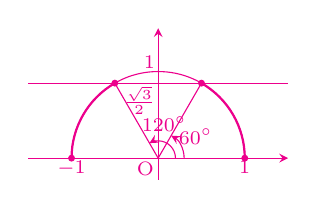
\begin{tikzpicture}[scale=1.1,color=magenta,>=stealth,]
        \node[below left=-2pt,font=\scriptsize] at (0,0){O}; 
        \node[above left,inner sep=1pt,font=\scriptsize] at (0,1){$1$}; 
        \node[below,inner sep=1pt,font=\scriptsize] at (1,0){$1$}; 
        \node[below,inner sep=1pt,font=\scriptsize] at (-1,0){$-1$}; 

        \draw[->] (-1.5,0) -- (1.5,0);
        \draw[->] (0,-0.25) -- (0,1.5);

        \draw (1,0) arc (0:180:1);

        \draw (-1.5,{0.5*sqrt(3)}) -- (1.5,{0.5*sqrt(3)});
        \node[below left=,inner sep=1pt,font=\scriptsize] at (0,{0.5*sqrt(3)}){$\frac{\sqrt{3}}{2}$};

        \coordinate (P1) at (60:1);
        \coordinate (P2) at (120:1);
        \fill (P1) circle[radius=0.4mm];
        \fill (P2) circle[radius=0.4mm];

        \draw (P1) -- (0,0);
        \draw (P2) -- (0,0);

        \draw[->] (0.3,0) arc (0:60:0.3);
        \draw[->] (0.2,0) arc (0:120:0.2);

        \node[font=\scriptsize]at (30:0.5) {$60^{\circ}$};
        \node[font=\scriptsize]at (80:0.4) {$120^{\circ}$};

        \draw[thick] (0:1) arc (0:60:1);
        \draw[thick] (120:1) arc (120:180:1);
        \fill (1,0) circle[radius=0.4mm];
        \fill (-1,0) circle[radius=0.4mm];
      \end{tikzpicture}
    \end{center}
    \item 下の図から$0^{\circ}\leq \theta<45^{\circ}$.
    \begin{center}
      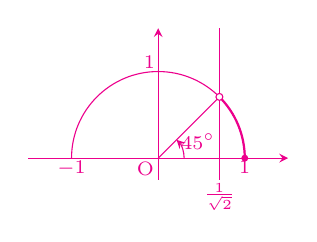
\begin{tikzpicture}[scale=1.1,color=magenta,>=stealth,]
        \node[below left=-2pt,font=\scriptsize] at (0,0){O}; 
        \node[above left,inner sep=1pt,font=\scriptsize] at (0,1){$1$}; 
        \node[below,inner sep=1pt,font=\scriptsize] at (1,0){$1$}; 
        \node[below,inner sep=1pt,font=\scriptsize] at (-1,0){$-1$}; 

        \draw[->] (-1.5,0) -- (1.5,0);
        \draw[->] (0,-0.25) -- (0,1.5);

        \draw (1,0) arc (0:180:1);

        \draw ({0.5*sqrt(2)},1.5) -- ({0.5*sqrt(2)},-0.25) node[below,inner sep=1pt,font=\scriptsize]{$\frac{1}{\sqrt{2}}$};

        \draw[thick] (0:1) arc (0:45:1);

        \coordinate (P1) at (0:1);
        \coordinate (P2) at (45:1);


        \draw (P2) -- (0,0);

        \draw[->] (0.3,0) arc (0:45:0.3);

        \node[font=\scriptsize]at (22.5:0.5) {$45^{\circ}$};
        % \node[font=\scriptsize]at (80:0.4) {$120^{\circ}$};

        \fill (P1) circle[radius=0.4mm];
        \filldraw[fill=white] (P2) circle[radius=0.4mm];
      \end{tikzpicture}
    \end{center}
    \item 下の図から$30^{\circ}\leq \theta< 90^{\circ}$.
    \begin{center}
      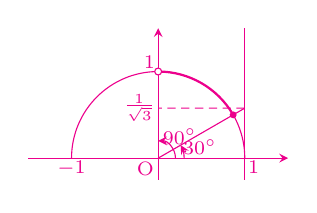
\begin{tikzpicture}[scale=1.1,color=magenta,>=stealth,]
        \node[below left=-2pt,font=\scriptsize] at (0,0){O}; 
        \node[above left,inner sep=1pt,font=\scriptsize] at (0,1){$1$}; 
        \node[below right,inner sep=1pt,font=\scriptsize] at (1,0){$1$}; 
        \node[below,inner sep=1pt,font=\scriptsize] at (-1,0){$-1$}; 

        \draw[->] (-1.5,0) -- (1.5,0);
        \draw[->] (0,-0.25) -- (0,1.5);

        \draw (1,0) arc (0:180:1);

        \draw (1,1.5) -- (1,-0.25);

        \coordinate (P1) at (1,{1/sqrt(3)});
        \coordinate (P2) at (90:1);
        \draw[densely dashed] (P1) -- (0,{1/sqrt(3)}) node[left,inner sep=1pt,font=\scriptsize]{$\frac{1}{\sqrt{3}}$};

        \draw[thick] (30:1) arc (30:90:1);
        
        \fill (30:1) circle[radius=0.4mm];
        \filldraw[fill=white] (P2) circle[radius=0.4mm];

        \draw (P1) -- (0,0);


        \draw[->] (0.3,0) arc (0:30:0.3);
        \draw[->] (0.2,0) arc (0:90:0.2);


        \node[font=\scriptsize]at (15:0.5) {$30^{\circ}$};
        \node[font=\scriptsize]at (45:0.35) {$90^{\circ}$};

      \end{tikzpicture}
    \end{center}
  \end{enumerate}
\end{解答挿入}

\newcolumn


\begin{問題挿入}[-1]{\themondai}<標準>
  $0^{\circ}\leq \theta\leq 180^{\circ}$のとき，次の方程式・不等式を解け。
  \begin{enumerate}
    \item $2\cos^{2}{\theta}+\sin{\theta}-1=0$
    \item $4\sin^{2}{\theta}+(2-2\sqrt{3})\cos{\theta}+\sqrt{3}-4\leq 0$
  \end{enumerate}
\end{問題挿入}
\begin{解答挿入}
  \begin{enumerate}
    \item 与えられた方程式から
    \begin{align*}
      2(1-\sin^2{\theta})+\sin{\theta}-1&=0 \\
      2\sin^{2}{\theta}-\sin{\theta}-1&=0 \\
      (\sin{\theta}-1)(2\sin{\theta}+1)&=0 \\
      \sin{\theta}&=1,\; -\frac{1}{2}
    \end{align*}
    を得る。\par
    $0^{\circ}\leq \theta\leq 180^{\circ}$より$0\leq \sin{\theta}\leq 1$であるから，$\sin{\theta}=-\frac{1}{2}$を満たす$\theta$の値は存在しない。\par
    ゆえに，下の図から解は\hspace{1\zw}$\theta=90^{\circ}$.
    \begin{center}
      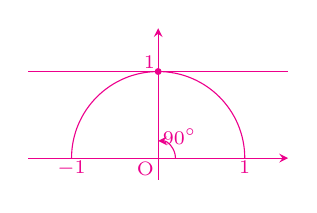
\begin{tikzpicture}[scale=1.1,color=magenta,>=stealth,]
        \node[below left=-2pt,font=\scriptsize] at (0,0){O}; 
        \node[above left,inner sep=1pt,font=\scriptsize] at (0,1){$1$}; 
        \node[below,inner sep=1pt,font=\scriptsize] at (1,0){$1$}; 
        \node[below,inner sep=1pt,font=\scriptsize] at (-1,0){$-1$}; 

        \draw[->] (-1.5,0) -- (1.5,0);
        \draw[->] (0,-0.25) -- (0,1.5);

        \draw (1,0) arc (0:180:1);

        \draw (-1.5,1) -- (1.5,1);

        \coordinate (P1) at (90:1);
        \fill (P1) circle[radius=0.4mm];

        \draw (P1) -- (0,0);

        \draw[->] (0.2,0) arc (0:90:0.2);

        \node[font=\scriptsize]at (45:0.35) {$90^{\circ}$};

      \end{tikzpicture}
    \end{center}
    \item 与えられた不等式から
    \begin{align*}
      4(1-\cos^2{\theta})+(2-2\sqrt{3})\cos{\theta}+\sqrt{3}-4&\leq 0 \\
      % -4\cos^{2}{\theta}+(2-2\sqrt{3})\cos{\theta}+\sqrt{3}&\leq 0 \\
      4\cos^{2}{\theta}+(2\sqrt{3}-2)\cos{\theta}-\sqrt{3}&\geq 0 \\
      (2\cos{\theta}-1)(2\cos{\theta}+\sqrt{3})&\geq 0
    \end{align*}
    より
    \begin{align*}
      \cos{\theta}\leq -\frac{\sqrt{3}}{2},\; \frac{1}{2}\leq\cos{\theta}
    \end{align*}
    を得る。\par
    ゆえに，下の図から解は\hspace{1\zw}$0^{\circ}\leq\theta\leq 60^{\circ},\; 150^{\circ}\leq\theta\leq 180^{\circ}$.
    \begin{center}
      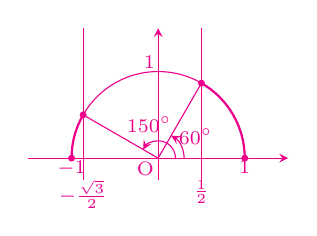
\begin{tikzpicture}[scale=1.1,color=magenta,>=stealth,]
        \node[below left=-2pt,font=\scriptsize] at (0,0){O}; 
        \node[above left,inner sep=1pt,font=\scriptsize] at (0,1){$1$}; 
        \node[below,inner sep=1pt,font=\scriptsize] at (1,0){$1$}; 
        \node[below,inner sep=1pt,font=\scriptsize] at (-1,0){$-1$}; 

        \draw[->] (-1.5,0) -- (1.5,0);
        \draw[->] (0,-0.25) -- (0,1.5);

        \draw (1,0) arc (0:180:1);

        \draw (0.5,1.5) -- (0.5,-0.25) node[below,inner sep=0pt,font=\scriptsize]{$\frac{1}{2}$};
        \draw ({-0.5*sqrt(3)},1.5) -- ({-0.5*sqrt(3)},-0.25) node[below,inner sep=0pt,font=\scriptsize]{$-\frac{\sqrt{3}}{2}$};

        \coordinate (P1) at (60:1);
        \coordinate (P2) at (150:1);
        \fill (P1) circle[radius=0.4mm];
        \fill (P2) circle[radius=0.4mm];

        \draw (P1) -- (0,0);
        \draw (P2) -- (0,0);

        \draw[->] (0.3,0) arc (0:60:0.3);
        \draw[->] (0.2,0) arc (0:150:0.2);

        \node[font=\scriptsize]at (30:0.5) {$60^{\circ}$};
        \node[font=\scriptsize]at (105:0.4) {$150^{\circ}$};

        \draw[thick] (0:1) arc (0:60:1);
        \draw[thick] (150:1) arc (150:180:1);

        \fill (1,0) circle[radius=0.4mm];
        \fill (-1,0) circle[radius=0.4mm];
      \end{tikzpicture}
    \end{center}
  \end{enumerate}
\end{解答挿入}

\end{分割}
\end{document}
